% Generated by Sphinx.
\def\sphinxdocclass{report}
\documentclass[letterpaper,10pt,openany,oneside]{sphinxmanual}
\usepackage[utf8]{inputenc}
\DeclareUnicodeCharacter{00A0}{\nobreakspace}
\usepackage[T1]{fontenc}
\usepackage[english]{babel}
\usepackage{times}
\usepackage[Bjarne]{fncychap}
\usepackage{longtable}
\usepackage{sphinx}
\usepackage{multirow}


\title{Optimizing CUDA for GPU Architecture}
\date{August 12, 2014}
\release{}
\author{CSInParallel Project}
\newcommand{\sphinxlogo}{}
\renewcommand{\releasename}{}
\makeindex

\makeatletter
\def\PYG@reset{\let\PYG@it=\relax \let\PYG@bf=\relax%
    \let\PYG@ul=\relax \let\PYG@tc=\relax%
    \let\PYG@bc=\relax \let\PYG@ff=\relax}
\def\PYG@tok#1{\csname PYG@tok@#1\endcsname}
\def\PYG@toks#1+{\ifx\relax#1\empty\else%
    \PYG@tok{#1}\expandafter\PYG@toks\fi}
\def\PYG@do#1{\PYG@bc{\PYG@tc{\PYG@ul{%
    \PYG@it{\PYG@bf{\PYG@ff{#1}}}}}}}
\def\PYG#1#2{\PYG@reset\PYG@toks#1+\relax+\PYG@do{#2}}

\expandafter\def\csname PYG@tok@gd\endcsname{\def\PYG@tc##1{\textcolor[rgb]{0.63,0.00,0.00}{##1}}}
\expandafter\def\csname PYG@tok@gu\endcsname{\let\PYG@bf=\textbf\def\PYG@tc##1{\textcolor[rgb]{0.50,0.00,0.50}{##1}}}
\expandafter\def\csname PYG@tok@gt\endcsname{\def\PYG@tc##1{\textcolor[rgb]{0.00,0.25,0.82}{##1}}}
\expandafter\def\csname PYG@tok@gs\endcsname{\let\PYG@bf=\textbf}
\expandafter\def\csname PYG@tok@gr\endcsname{\def\PYG@tc##1{\textcolor[rgb]{1.00,0.00,0.00}{##1}}}
\expandafter\def\csname PYG@tok@cm\endcsname{\let\PYG@it=\textit\def\PYG@tc##1{\textcolor[rgb]{0.25,0.50,0.56}{##1}}}
\expandafter\def\csname PYG@tok@vg\endcsname{\def\PYG@tc##1{\textcolor[rgb]{0.73,0.38,0.84}{##1}}}
\expandafter\def\csname PYG@tok@m\endcsname{\def\PYG@tc##1{\textcolor[rgb]{0.13,0.50,0.31}{##1}}}
\expandafter\def\csname PYG@tok@mh\endcsname{\def\PYG@tc##1{\textcolor[rgb]{0.13,0.50,0.31}{##1}}}
\expandafter\def\csname PYG@tok@cs\endcsname{\def\PYG@tc##1{\textcolor[rgb]{0.25,0.50,0.56}{##1}}\def\PYG@bc##1{\setlength{\fboxsep}{0pt}\colorbox[rgb]{1.00,0.94,0.94}{\strut ##1}}}
\expandafter\def\csname PYG@tok@ge\endcsname{\let\PYG@it=\textit}
\expandafter\def\csname PYG@tok@vc\endcsname{\def\PYG@tc##1{\textcolor[rgb]{0.73,0.38,0.84}{##1}}}
\expandafter\def\csname PYG@tok@il\endcsname{\def\PYG@tc##1{\textcolor[rgb]{0.13,0.50,0.31}{##1}}}
\expandafter\def\csname PYG@tok@go\endcsname{\def\PYG@tc##1{\textcolor[rgb]{0.19,0.19,0.19}{##1}}}
\expandafter\def\csname PYG@tok@cp\endcsname{\def\PYG@tc##1{\textcolor[rgb]{0.00,0.44,0.13}{##1}}}
\expandafter\def\csname PYG@tok@gi\endcsname{\def\PYG@tc##1{\textcolor[rgb]{0.00,0.63,0.00}{##1}}}
\expandafter\def\csname PYG@tok@gh\endcsname{\let\PYG@bf=\textbf\def\PYG@tc##1{\textcolor[rgb]{0.00,0.00,0.50}{##1}}}
\expandafter\def\csname PYG@tok@ni\endcsname{\let\PYG@bf=\textbf\def\PYG@tc##1{\textcolor[rgb]{0.84,0.33,0.22}{##1}}}
\expandafter\def\csname PYG@tok@nl\endcsname{\let\PYG@bf=\textbf\def\PYG@tc##1{\textcolor[rgb]{0.00,0.13,0.44}{##1}}}
\expandafter\def\csname PYG@tok@nn\endcsname{\let\PYG@bf=\textbf\def\PYG@tc##1{\textcolor[rgb]{0.05,0.52,0.71}{##1}}}
\expandafter\def\csname PYG@tok@no\endcsname{\def\PYG@tc##1{\textcolor[rgb]{0.38,0.68,0.84}{##1}}}
\expandafter\def\csname PYG@tok@na\endcsname{\def\PYG@tc##1{\textcolor[rgb]{0.25,0.44,0.63}{##1}}}
\expandafter\def\csname PYG@tok@nb\endcsname{\def\PYG@tc##1{\textcolor[rgb]{0.00,0.44,0.13}{##1}}}
\expandafter\def\csname PYG@tok@nc\endcsname{\let\PYG@bf=\textbf\def\PYG@tc##1{\textcolor[rgb]{0.05,0.52,0.71}{##1}}}
\expandafter\def\csname PYG@tok@nd\endcsname{\let\PYG@bf=\textbf\def\PYG@tc##1{\textcolor[rgb]{0.33,0.33,0.33}{##1}}}
\expandafter\def\csname PYG@tok@ne\endcsname{\def\PYG@tc##1{\textcolor[rgb]{0.00,0.44,0.13}{##1}}}
\expandafter\def\csname PYG@tok@nf\endcsname{\def\PYG@tc##1{\textcolor[rgb]{0.02,0.16,0.49}{##1}}}
\expandafter\def\csname PYG@tok@si\endcsname{\let\PYG@it=\textit\def\PYG@tc##1{\textcolor[rgb]{0.44,0.63,0.82}{##1}}}
\expandafter\def\csname PYG@tok@s2\endcsname{\def\PYG@tc##1{\textcolor[rgb]{0.25,0.44,0.63}{##1}}}
\expandafter\def\csname PYG@tok@vi\endcsname{\def\PYG@tc##1{\textcolor[rgb]{0.73,0.38,0.84}{##1}}}
\expandafter\def\csname PYG@tok@nt\endcsname{\let\PYG@bf=\textbf\def\PYG@tc##1{\textcolor[rgb]{0.02,0.16,0.45}{##1}}}
\expandafter\def\csname PYG@tok@nv\endcsname{\def\PYG@tc##1{\textcolor[rgb]{0.73,0.38,0.84}{##1}}}
\expandafter\def\csname PYG@tok@s1\endcsname{\def\PYG@tc##1{\textcolor[rgb]{0.25,0.44,0.63}{##1}}}
\expandafter\def\csname PYG@tok@gp\endcsname{\let\PYG@bf=\textbf\def\PYG@tc##1{\textcolor[rgb]{0.78,0.36,0.04}{##1}}}
\expandafter\def\csname PYG@tok@sh\endcsname{\def\PYG@tc##1{\textcolor[rgb]{0.25,0.44,0.63}{##1}}}
\expandafter\def\csname PYG@tok@ow\endcsname{\let\PYG@bf=\textbf\def\PYG@tc##1{\textcolor[rgb]{0.00,0.44,0.13}{##1}}}
\expandafter\def\csname PYG@tok@sx\endcsname{\def\PYG@tc##1{\textcolor[rgb]{0.78,0.36,0.04}{##1}}}
\expandafter\def\csname PYG@tok@bp\endcsname{\def\PYG@tc##1{\textcolor[rgb]{0.00,0.44,0.13}{##1}}}
\expandafter\def\csname PYG@tok@c1\endcsname{\let\PYG@it=\textit\def\PYG@tc##1{\textcolor[rgb]{0.25,0.50,0.56}{##1}}}
\expandafter\def\csname PYG@tok@kc\endcsname{\let\PYG@bf=\textbf\def\PYG@tc##1{\textcolor[rgb]{0.00,0.44,0.13}{##1}}}
\expandafter\def\csname PYG@tok@c\endcsname{\let\PYG@it=\textit\def\PYG@tc##1{\textcolor[rgb]{0.25,0.50,0.56}{##1}}}
\expandafter\def\csname PYG@tok@mf\endcsname{\def\PYG@tc##1{\textcolor[rgb]{0.13,0.50,0.31}{##1}}}
\expandafter\def\csname PYG@tok@err\endcsname{\def\PYG@bc##1{\setlength{\fboxsep}{0pt}\fcolorbox[rgb]{1.00,0.00,0.00}{1,1,1}{\strut ##1}}}
\expandafter\def\csname PYG@tok@kd\endcsname{\let\PYG@bf=\textbf\def\PYG@tc##1{\textcolor[rgb]{0.00,0.44,0.13}{##1}}}
\expandafter\def\csname PYG@tok@ss\endcsname{\def\PYG@tc##1{\textcolor[rgb]{0.32,0.47,0.09}{##1}}}
\expandafter\def\csname PYG@tok@sr\endcsname{\def\PYG@tc##1{\textcolor[rgb]{0.14,0.33,0.53}{##1}}}
\expandafter\def\csname PYG@tok@mo\endcsname{\def\PYG@tc##1{\textcolor[rgb]{0.13,0.50,0.31}{##1}}}
\expandafter\def\csname PYG@tok@mi\endcsname{\def\PYG@tc##1{\textcolor[rgb]{0.13,0.50,0.31}{##1}}}
\expandafter\def\csname PYG@tok@kn\endcsname{\let\PYG@bf=\textbf\def\PYG@tc##1{\textcolor[rgb]{0.00,0.44,0.13}{##1}}}
\expandafter\def\csname PYG@tok@o\endcsname{\def\PYG@tc##1{\textcolor[rgb]{0.40,0.40,0.40}{##1}}}
\expandafter\def\csname PYG@tok@kr\endcsname{\let\PYG@bf=\textbf\def\PYG@tc##1{\textcolor[rgb]{0.00,0.44,0.13}{##1}}}
\expandafter\def\csname PYG@tok@s\endcsname{\def\PYG@tc##1{\textcolor[rgb]{0.25,0.44,0.63}{##1}}}
\expandafter\def\csname PYG@tok@kp\endcsname{\def\PYG@tc##1{\textcolor[rgb]{0.00,0.44,0.13}{##1}}}
\expandafter\def\csname PYG@tok@w\endcsname{\def\PYG@tc##1{\textcolor[rgb]{0.73,0.73,0.73}{##1}}}
\expandafter\def\csname PYG@tok@kt\endcsname{\def\PYG@tc##1{\textcolor[rgb]{0.56,0.13,0.00}{##1}}}
\expandafter\def\csname PYG@tok@sc\endcsname{\def\PYG@tc##1{\textcolor[rgb]{0.25,0.44,0.63}{##1}}}
\expandafter\def\csname PYG@tok@sb\endcsname{\def\PYG@tc##1{\textcolor[rgb]{0.25,0.44,0.63}{##1}}}
\expandafter\def\csname PYG@tok@k\endcsname{\let\PYG@bf=\textbf\def\PYG@tc##1{\textcolor[rgb]{0.00,0.44,0.13}{##1}}}
\expandafter\def\csname PYG@tok@se\endcsname{\let\PYG@bf=\textbf\def\PYG@tc##1{\textcolor[rgb]{0.25,0.44,0.63}{##1}}}
\expandafter\def\csname PYG@tok@sd\endcsname{\let\PYG@it=\textit\def\PYG@tc##1{\textcolor[rgb]{0.25,0.44,0.63}{##1}}}

\def\PYGZbs{\char`\\}
\def\PYGZus{\char`\_}
\def\PYGZob{\char`\{}
\def\PYGZcb{\char`\}}
\def\PYGZca{\char`\^}
\def\PYGZam{\char`\&}
\def\PYGZlt{\char`\<}
\def\PYGZgt{\char`\>}
\def\PYGZsh{\char`\#}
\def\PYGZpc{\char`\%}
\def\PYGZdl{\char`\$}
\def\PYGZti{\char`\~}
% for compatibility with earlier versions
\def\PYGZat{@}
\def\PYGZlb{[}
\def\PYGZrb{]}
\makeatother

\begin{document}

\maketitle
\tableofcontents
\phantomsection\label{index::doc}


nVIDIA GPU cards use an advanced arcitecture to efficiently execute
massively parallel programs written in CUDA C. This module explains how to take
advantage of this architecture to provide maximum speedup for
your CUDA applications using a mandelbrot set generator as an
example. It is intended to be a resource for instructors wishing
to create lectures, though it can also be presented to students
as is.

Feel free to use and modify the code and images in this module
in your lectures.

\emph{created by Jeffrey Lyman 2014 JLyman@macalester.edu}


\chapter{CUDA Architecture}
\label{0-Architecture/Architecture:optimizing-cuda-for-gpu-architecture}\label{0-Architecture/Architecture::doc}\label{0-Architecture/Architecture:cuda-architecture}
CPUs are designed to process as many sequential instructions as
quickly as possible. While most CPUs support threading, creating
a thread is usually an expensive operation and high-end CPUs can
usually make efficient use of no more than about 12 concurrent threads.

GPUs on the other hand are designed to process a small number of
parallel instructions on large sets of data as quickly as
possible. For instance, calculating 1 million polygons and
determining which to draw on the screen and where. To do this they
rely on many slower processors and inexpensive threads.


\section{Physical Architecture}
\label{0-Architecture/Architecture:physical-architecture}
CUDA-capable GPU cards are composed of one or more \textbf{Streaming Multiprocessors}
(SMs), which are an abstraction of the underlying hardware.
Each SM has a set of \textbf{Streaming Processors} (SPs), also called CUDA cores, which share a cache of shared memory
that is faster than the GPU's global memory but that can only be accessed by the threads
running on the SPs the that SM.  These streaming processors are the ``cores'' that
execute instructions.

The numbers of SPs/cores in an SM and the number of SMs depend on your device: see the \emph{Finding your
Device Specifications} section below for details. It is important to realize, however, that
regardless of GPU model, there are many more CUDA cores in a GPU than in a typical multicore CPU:
hundreds or thousands more. For example, the Kepler Streaming Multiprocessor design, dubbed SMX, contains 192
single-precision CUDA cores, 64 double-precision units, 32 special function units, and 32 load/store units.
(See the \href{http://www.nvidia.com/content/PDF/kepler/NVIDIA-Kepler-GK110-Architecture-Whitepaper.pdf}{Kepler Architecture Whitepaper}
for a description and diagram.)

CUDA cores are grouped together to perform instructions in
a what nVIDIA has termed a \textbf{warp} of threads. Warp simply means a group of threads
that are scheduled together to execute the same instructions in lockstep.
All CUDA cards to date use a warp size of 32.
Each SM has at least one warp scheduler, which is responsible for executing 32 threads.
Depending on the model of GPU, the cores may be
double or quadruple pumped so that they execute one instruction
on two or four threads in as many clock cycles.
For instance, Tesla devices use a group of 8 quadpumped cores
to execute a single warp. If there are less than 32 threads scheduled in
the warp, it will still take as long to execute the instructions.

The CUDA programmer is responsible for ensuring that the threads are being assigned
efficiently for code that is designed to run on the GPU.  The assignment of threads
is done virtually in the code using what is sometimes referred to as a `tiling' scheme
of blocks of threads that form a grid.  Programmers define a \textbf{kernel function}
that will be executed on the CUDA card using a particular tiling scheme.


\section{Virtual Architecture}
\label{0-Architecture/Architecture:virtual-architecture}
When programming in CUDA C we work with blocks of threads and
grids of blocks. What is the relationship between this virtual
architecture and the CUDA card's physical architecture?

When kernels are launched, each block in a grid is assigned to a
Streaming Multiprocessor. This allows threads in a block to use
\code{\_\_shared\_\_} memory. If a block doesn't use the full resources
of the SM then multiple blocks may be assigned at once. If all of
the SMs are busy then the extra blocks will have to wait until a
SM becomes free.

Once a block is assigned to an SM, it's threads are split into
warps by the warp scheduler and executed on the CUDA cores.
Since the same instructions are executed on each thread in the
warp simultaneously it's generally a bad idea to have
conditionals in kernel code.  This type of code is sometimes called \emph{divergent}:
when some threads in a warp are unable to execute the same instruction
as other threads in a warp, those threads are diverged and do no work.

Because a warp's context (it's registers, program counter etc.)
stays on chip for the life of the warp, there is no additional
cost to switching between warps vs executing the next step of a
given warp. This allows the GPU to switch to hide some of it's
memory latency by switching to a new warp while it waits for a
costly read.


\section{CUDA Memory}
\label{0-Architecture/Architecture:cuda-memory}
CUDA on chip memory is divided into several different regions
\begin{itemize}
\item {} \begin{description}
\item[{\textbf{Registers} act the same way that registers on CPUs do, each}] \leavevmode
thread has it's own set of registers.

\end{description}

\item {} \begin{description}
\item[{\textbf{Local Memory} local variables used by each thread. They are}] \leavevmode
not accesible by other threads even though they use the same
L1 and L2 cache as global memory.

\end{description}

\item {} \begin{description}
\item[{\textbf{Shared Memory} is accessible by all threads in a block. It}] \leavevmode
must be declared using the \code{\_\_shared\_\_} modifier. It has a
higher bandwidth and lower latency than global memory. However, if
multiple threads request the same address, the requests are
processed serially, which slows down the application.

\end{description}

\item {} \begin{description}
\item[{\textbf{Constant Memory} is read-accessible by all theads and must}] \leavevmode
be declared with the \code{\_\_const\_\_} modifier. In newer devices
there is a seperate read only constant cache.

\end{description}

\item {} \begin{description}
\item[{\textbf{Global Memory} is accessible by all threads. It's the}] \leavevmode
slowest device memory, but on new cards, it is cached. Memory
is pulled in 32, 64, or 128 byte memory transactions. Warps
executing global memory accesses attempt to pull all the data
from global memory simultaneously therefore it's advantageous
to use block sizes that are multiples of 32. If
multidimensional arrays are used, it's also advantageous to
have the bounds padded so that they are multiples of 32

\end{description}

\item {} \begin{description}
\item[{\textbf{Texture/Surface Memory} is read-accesible by all threads, but}] \leavevmode
unlike Constant Memory, it is optimized for 2D spacial
locality, and cache hits pull in surrounding values in both
x and y directions.

\end{description}

\end{itemize}
\begin{figure}[htbp]
\centering
\capstart

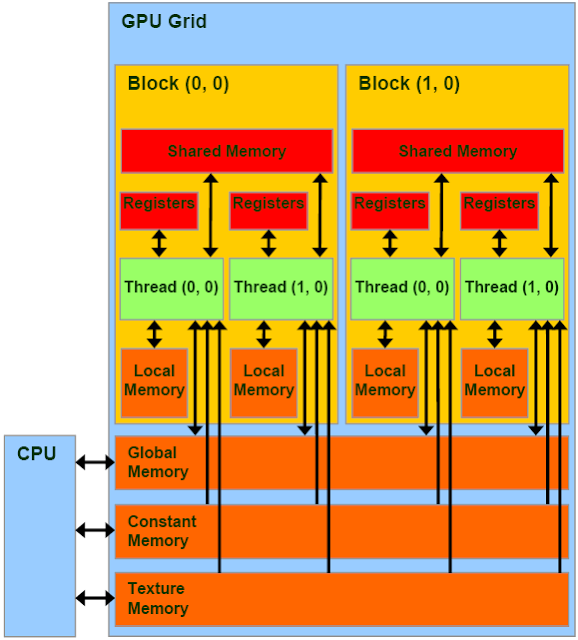
\includegraphics{memheirarchy.png}
\caption{\emph{CUDA Memory Hierarchy}
\emph{Image courtesy of NVIDIA}}\end{figure}


\section{Finding your Device Specifications}
\label{0-Architecture/Architecture:finding-your-device-specifications}
nVIDIA provides a program with the installation of the CUDA developer toolkit
that prints out the specifications of
your device. To run it on a unix machine, execute this command:

\code{/usr/local/cuda/samples/1\_Utilities/deviceQuery/deviceQuery}

If that doesn't work you probably need to build the samples

\begin{Verbatim}[commandchars=\\\{\}]
\PYG{n+nb}{cd} /usr/local/cuda/samples/1\PYGZus{}Utilities/deviceQuery
sudo make
./deviceQuery
\end{Verbatim}

Look for the number of Multiprocessors on your device,
the number of CUDA cores per SM, and the warp size.

The CUDA Toolkit with the samples is also available for Windows using Visual studio.
See the excellent and thorough \href{http://docs.nvidia.com/cuda/cuda-getting-started-guide-for-microsoft-windows/\#axzz3ACR56e2v}{Getting Started Guide for Windows}
provided by nVIDIA for more information.  However, some of the code described in the
next section uses X11 calls for its graphical display, which will not easily run in Windows.
You will need a package like Cygwin/X.


\chapter{Mandelbrot Test Code}
\label{1-Mandelbrot/Mandelbrot:mandelbrot-test-code}\label{1-Mandelbrot/Mandelbrot::doc}
Choosing a good number of blocks and threads per block is
an important part of CUDA Programming. To illustrate this, we
will take a look at a program that generates images of the
Mandelbrot set. To run the programs you will need a CUDA capable
machine as well as the appropriate XOrg
developer package (X11 is likely installed on your linux machine
and needs to be installed on a Mac). Download \code{mandelbrot.cu} and the
\code{Makefile} and run \code{make all} This will generate 3
programs:

\textbf{Mandelbrot} is a mandelbrot set viewer designed for demonstrations
. It allows you to zoom in and out and move around the
Mandelbrot set. The controls are w for up, s for down, a for
left, d for right, e to zoom in, q to zoom out and x to exit.

The executable named \textbf{benchmark} runs the computation without displaying anything and
prints out the time it took before exiting.

\textbf{XBenchmark} is a hybrid that prints out the computation time and
allows you to move around. This is useful because the computation
time is dependent on your position within the Mandelbrot set.

Each of the programs takes betwen 0 and 4 commandline arguments
\begin{enumerate}
\item {} 
the number of blocks used by the kernel

\item {} 
the number of threads per block

\item {} 
the image size in pixels, the image is always square

\item {} 
the image depth (explained later)

\end{enumerate}


\section{What is the Mandelbrot set?}
\label{1-Mandelbrot/Mandelbrot:what-is-the-mandelbrot-set}
The mandelbrot set is defined as the set of all complex numbers C
such that the formula Z$_{\text{n+1}}$ = Z$_{\text{n}}$$^{\text{2}}$ + C
tends towards infinity. If we plot the real values of C on the X
axis and the imaginary values of C on the Y axis we get a two
dimensional fractal shape, such as this one created from running this code.
\begin{figure}[htbp]
\centering


\includegraphics{set.jpg}
\end{figure}


\section{Coding the Mandelbrot set}
\label{1-Mandelbrot/Mandelbrot:coding-the-mandelbrot-set}
The to determine whether a value is in or out of the mandelbrot
set we loop through the formula  Z$_{\text{n+1}}$ = Z$_{\text{n}}$$^{\text{2}}$ + C a certain number of times (this is the image depth
from earlier) and during each iteration, check if the magnitude
of Z is greater than 2; if so, we return false. However we want our
Mandelbrot image to look pretty, so instead we'll return the
iteration in which it went out of bounds and and then interpret
that number as a color. If it completes the loop without going
out of bounds we'll assign it the color black

After some algebraic manipulation to reduce the number of
floating point multiplications, our code looks like this:

\begin{Verbatim}[commandchars=\\\{\}]
\PYG{n}{\PYGZus{}\PYGZus{}device\PYGZus{}\PYGZus{}} \PYG{k+kt}{uint32\PYGZus{}t} \PYG{n+nf}{mandel\PYGZus{}double}\PYG{p}{(}\PYG{k+kt}{double} \PYG{n}{cr}\PYG{p}{,} \PYG{k+kt}{double} \PYG{n}{ci}\PYG{p}{,} \PYG{k+kt}{int} \PYG{n}{max\PYGZus{}iter}\PYG{p}{)} \PYG{p}{\PYGZob{}}
    \PYG{k+kt}{double} \PYG{n}{zr} \PYG{o}{=} \PYG{l+m+mi}{0}\PYG{p}{;}
    \PYG{k+kt}{double} \PYG{n}{zi} \PYG{o}{=} \PYG{l+m+mi}{0}\PYG{p}{;}
    \PYG{k+kt}{double} \PYG{n}{zrsqr} \PYG{o}{=} \PYG{l+m+mi}{0}\PYG{p}{;}
    \PYG{k+kt}{double} \PYG{n}{zisqr} \PYG{o}{=} \PYG{l+m+mi}{0}\PYG{p}{;}

    \PYG{k+kt}{uint32\PYGZus{}t} \PYG{n}{i}\PYG{p}{;}

    \PYG{k}{for} \PYG{p}{(}\PYG{n}{i} \PYG{o}{=} \PYG{l+m+mi}{0}\PYG{p}{;} \PYG{n}{i} \PYG{o}{\PYGZlt{}} \PYG{n}{max\PYGZus{}iter}\PYG{p}{;} \PYG{n}{i}\PYG{o}{+}\PYG{o}{+}\PYG{p}{)}\PYG{p}{\PYGZob{}}
		\PYG{n}{zi} \PYG{o}{=} \PYG{n}{zr} \PYG{o}{*} \PYG{n}{zi}\PYG{p}{;}
		\PYG{n}{zi} \PYG{o}{+}\PYG{o}{=} \PYG{n}{zi}\PYG{p}{;}
		\PYG{n}{zi} \PYG{o}{+}\PYG{o}{=} \PYG{n}{ci}\PYG{p}{;}
		\PYG{n}{zr} \PYG{o}{=} \PYG{n}{zrsqr} \PYG{o}{-} \PYG{n}{zisqr} \PYG{o}{+} \PYG{n}{cr}\PYG{p}{;}
		\PYG{n}{zrsqr} \PYG{o}{=} \PYG{n}{zr} \PYG{o}{*} \PYG{n}{zr}\PYG{p}{;}
		\PYG{n}{zisqr} \PYG{o}{=} \PYG{n}{zi} \PYG{o}{*} \PYG{n}{zi}\PYG{p}{;}
		
    \PYG{c+c1}{//the fewer iterations it takes to diverge, the farther from the set}
		\PYG{k}{if} \PYG{p}{(}\PYG{n}{zrsqr} \PYG{o}{+} \PYG{n}{zisqr} \PYG{o}{\PYGZgt{}} \PYG{l+m+mf}{4.0}\PYG{p}{)} \PYG{k}{break}\PYG{p}{;}
    \PYG{p}{\PYGZcb{}}
	
    \PYG{k}{return} \PYG{n}{i}\PYG{p}{;}
\PYG{p}{\PYGZcb{}}
\end{Verbatim}
\setbox0\vbox{
\begin{minipage}{0.95\linewidth}
\textbf{Some notes about this CUDA code}

\medskip

\begin{itemize}
\item {} 
A function that is designed to be run on th GPU is designated with the special keyword \emph{\_\_device\_\_}.

\item {} 
The type uint32\_t is an unsigned 32-bit integer declared in stdint.h.

\item {} 
The variable max\_iter is defaulted to be 100, and can be changed with the image depth command line argument.

\end{itemize}
\end{minipage}}
\begin{center}\setlength{\fboxsep}{5pt}\shadowbox{\box0}\end{center}

But wait didn't we say in the last chapter that conditionals
should be avoided? Yes, when a thread returns early, it's
just dead weight in the warp, howerver due to the nature of
the mandelbrot set it is very likely
that some warps have threads that all terminate before
reaching \code{max\_iter} so in some cases it will give us a
slight speed up. If the warp contains a point within the
Mandelbrot set, we won't get any speed up from breaking.

We also need a kernel that will divide the pixels between
the threads and run \code{mandel\_double} on each of them
Our code is as follows where \code{dim} is the image dimension,
\code{counts} is the list representing our image, and \code{step}
represents the distance between the points represented by
the pixels:

\begin{Verbatim}[commandchars=\\\{\}]
\PYG{n}{\PYGZus{}\PYGZus{}global\PYGZus{}\PYGZus{}} \PYG{k+kt}{void} \PYG{n+nf}{mandel\PYGZus{}kernel}\PYG{p}{(}\PYG{k+kt}{uint32\PYGZus{}t} \PYG{o}{*}\PYG{n}{counts}\PYG{p}{,} \PYG{k+kt}{double} \PYG{n}{xmin}\PYG{p}{,} \PYG{k+kt}{double} \PYG{n}{ymin}\PYG{p}{,}
            \PYG{k+kt}{double} \PYG{n}{step}\PYG{p}{,} \PYG{k+kt}{int} \PYG{n}{max\PYGZus{}iter}\PYG{p}{,} \PYG{k+kt}{int} \PYG{n}{dim}\PYG{p}{,} \PYG{k+kt}{uint32\PYGZus{}t} \PYG{o}{*}\PYG{n}{colors}\PYG{p}{)} \PYG{p}{\PYGZob{}}
    \PYG{k+kt}{int} \PYG{n}{pix\PYGZus{}per\PYGZus{}thread} \PYG{o}{=} \PYG{n}{dim} \PYG{o}{*} \PYG{n}{dim} \PYG{o}{/} \PYG{p}{(}\PYG{n}{gridDim}\PYG{p}{.}\PYG{n}{x} \PYG{o}{*} \PYG{n}{blockDim}\PYG{p}{.}\PYG{n}{x}\PYG{p}{)}\PYG{p}{;}
    \PYG{k+kt}{int} \PYG{n}{tId} \PYG{o}{=} \PYG{n}{blockDim}\PYG{p}{.}\PYG{n}{x} \PYG{o}{*} \PYG{n}{blockIdx}\PYG{p}{.}\PYG{n}{x} \PYG{o}{+} \PYG{n}{threadIdx}\PYG{p}{.}\PYG{n}{x}\PYG{p}{;}
    \PYG{k+kt}{int} \PYG{n}{offset} \PYG{o}{=} \PYG{n}{pix\PYGZus{}per\PYGZus{}thread} \PYG{o}{*} \PYG{n}{tId}\PYG{p}{;}
    \PYG{k}{for} \PYG{p}{(}\PYG{k+kt}{int} \PYG{n}{i} \PYG{o}{=} \PYG{n}{offset}\PYG{p}{;} \PYG{n}{i} \PYG{o}{\PYGZlt{}} \PYG{n}{offset} \PYG{o}{+} \PYG{n}{pix\PYGZus{}per\PYGZus{}thread}\PYG{p}{;} \PYG{n}{i}\PYG{o}{+}\PYG{o}{+}\PYG{p}{)}\PYG{p}{\PYGZob{}}
        \PYG{k+kt}{int} \PYG{n}{x} \PYG{o}{=} \PYG{n}{i} \PYG{o}{\PYGZpc{}} \PYG{n}{dim}\PYG{p}{;}
        \PYG{k+kt}{int} \PYG{n}{y} \PYG{o}{=} \PYG{n}{i} \PYG{o}{/} \PYG{n}{dim}\PYG{p}{;}
        \PYG{k+kt}{double} \PYG{n}{cr} \PYG{o}{=} \PYG{n}{xmin} \PYG{o}{+} \PYG{n}{x} \PYG{o}{*} \PYG{n}{step}\PYG{p}{;}
        \PYG{k+kt}{double} \PYG{n}{ci} \PYG{o}{=} \PYG{n}{ymin} \PYG{o}{+} \PYG{n}{y} \PYG{o}{*} \PYG{n}{step}\PYG{p}{;}
        \PYG{n}{counts}\PYG{p}{[}\PYG{n}{y} \PYG{o}{*} \PYG{n}{dim} \PYG{o}{+} \PYG{n}{x}\PYG{p}{]}  \PYG{o}{=} \PYG{n}{colors}\PYG{p}{[}\PYG{n}{mandel\PYGZus{}double}\PYG{p}{(}\PYG{n}{cr}\PYG{p}{,} \PYG{n}{ci}\PYG{p}{,} \PYG{n}{max\PYGZus{}iter}\PYG{p}{)}\PYG{p}{]}\PYG{p}{;}
    \PYG{p}{\PYGZcb{}}
    \PYG{k}{if} \PYG{p}{(}\PYG{n}{gridDim}\PYG{p}{.}\PYG{n}{x} \PYG{o}{*} \PYG{n}{blockDim}\PYG{p}{.}\PYG{n}{x} \PYG{o}{*} \PYG{n}{pix\PYGZus{}per\PYGZus{}thread} \PYG{o}{\PYGZlt{}} \PYG{n}{dim} \PYG{o}{*} \PYG{n}{dim}
            \PYG{o}{\PYGZam{}}\PYG{o}{\PYGZam{}} \PYG{n}{tId} \PYG{o}{\PYGZlt{}} \PYG{p}{(}\PYG{n}{dim} \PYG{o}{*} \PYG{n}{dim}\PYG{p}{)} \PYG{o}{-} \PYG{p}{(}\PYG{n}{blockDim}\PYG{p}{.}\PYG{n}{x} \PYG{o}{*} \PYG{n}{gridDim}\PYG{p}{.}\PYG{n}{x}\PYG{p}{)}\PYG{p}{)}\PYG{p}{\PYGZob{}}
        \PYG{k+kt}{int} \PYG{n}{i} \PYG{o}{=} \PYG{n}{blockDim}\PYG{p}{.}\PYG{n}{x} \PYG{o}{*} \PYG{n}{gridDim}\PYG{p}{.}\PYG{n}{x} \PYG{o}{*} \PYG{n}{pix\PYGZus{}per\PYGZus{}thread} \PYG{o}{+} \PYG{n}{tId}\PYG{p}{;}
        \PYG{k+kt}{int} \PYG{n}{x} \PYG{o}{=} \PYG{n}{i} \PYG{o}{\PYGZpc{}} \PYG{n}{dim}\PYG{p}{;}
        \PYG{k+kt}{int} \PYG{n}{y} \PYG{o}{=} \PYG{n}{i} \PYG{o}{/} \PYG{n}{dim}\PYG{p}{;}
        \PYG{k+kt}{double} \PYG{n}{cr} \PYG{o}{=} \PYG{n}{xmin} \PYG{o}{+} \PYG{n}{x} \PYG{o}{*} \PYG{n}{step}\PYG{p}{;}
        \PYG{k+kt}{double} \PYG{n}{ci} \PYG{o}{=} \PYG{n}{ymin} \PYG{o}{+} \PYG{n}{y} \PYG{o}{*} \PYG{n}{step}\PYG{p}{;}
        \PYG{n}{counts}\PYG{p}{[}\PYG{n}{y} \PYG{o}{*} \PYG{n}{dim} \PYG{o}{+} \PYG{n}{x}\PYG{p}{]}  \PYG{o}{=} \PYG{n}{colors}\PYG{p}{[}\PYG{n}{mandel\PYGZus{}double}\PYG{p}{(}\PYG{n}{cr}\PYG{p}{,} \PYG{n}{ci}\PYG{p}{,} \PYG{n}{max\PYGZus{}iter}\PYG{p}{)}\PYG{p}{]}\PYG{p}{;}
    \PYG{p}{\PYGZcb{}}
    
\PYG{p}{\PYGZcb{}}
\end{Verbatim}
\setbox0\vbox{
\begin{minipage}{0.95\linewidth}
\textbf{Some notes about this CUDA code}

\medskip

\begin{itemize}
\item {} 
The keyword \emph{\_\_global\_\_} designates the kernel function.

\item {} 
We execute the kernel function on the GPU device from main() like this, where \emph{n} is the number of blocks of threads and `m' is the number of threads per block:

\end{itemize}

\begin{Verbatim}[commandchars=\\\{\}]
    \PYG{n}{mandel\PYGZus{}kernel}\PYG{o}{\PYGZlt{}}\PYG{o}{\PYGZlt{}}\PYG{o}{\PYGZlt{}}\PYG{n}{n}\PYG{p}{,} \PYG{n}{m}\PYG{o}{\PYGZgt{}}\PYG{o}{\PYGZgt{}}\PYG{o}{\PYGZgt{}}\PYG{p}{(}\PYG{n}{dev\PYGZus{}counts}\PYG{p}{,} \PYG{n}{xmin} \PYG{p}{,} \PYG{n}{ymin}\PYG{p}{,} \PYG{n}{step}\PYG{p}{,} \PYG{n}{max\PYGZus{}iter}\PYG{p}{,} \PYG{n}{dim}\PYG{p}{,} \PYG{n}{colors}\PYG{p}{)}\PYG{p}{;}
\end{Verbatim}
\begin{itemize}
\item {} 
In this case, the `tiling' of the blocks of threads into a grid is a one-dimensional array of n blocks.

\item {} 
Each thread calculates a particular value in the set based on its thread id (tId in the above code), which can be calculated using a data structure called \emph{blockDim}, along with ones called \emph{blockIdx} and \emph{threadIdx}. The value blockDim.x gives us the total number of threads per block. The blockIdx.x value gives us the index of the block in which a particular thread running this code is located.  Lastly, the threadIdx.x value is the index of this thread in its block. Thus, a thread running this code can uniquely identify itself with the computation \emph{blockDim.x * blockIdx.x + threadIdx.x}.

\item {} 
We use blockDim.x when calculating the thread id above so that we could change the number of blocks, n, and the number of threads per block, m, programatically with command-line arguments and not have to change the lernel function.

\end{itemize}
\end{minipage}}
\begin{center}\setlength{\fboxsep}{5pt}\shadowbox{\box0}\end{center}

In order to compensate for block and grid dimensions that
do not easily divide the picture we make the first threads
pick up the `slack.' This is also the reason why we are not
using 2 dimensional grids and blocks.

\begin{notice}{warning}{Warning:}
Always try to make your threads do the same amount of work.
Scheduling extra work for some threads is inefficient since
the other threads in the warp will have to wait for them to
finish anyway. This code is purposefully messy so that it
runs for any problem size.
\end{notice}

That's the meat of the program, feel free to explore the
it on your own, most of the rest of the program is dedicated to
displaying the data generated by these 2 functions.

In the next section, we will discuss how to choose the number of
blocks and the number of threads per block in order to take maximum advantage of
the GPU hardware.


\chapter{Choosing the right Dimensions}
\label{2-Findings/Findings:choosing-the-right-dimensions}\label{2-Findings/Findings::doc}\setbox0\vbox{
\begin{minipage}{0.95\linewidth}
\textbf{Compute Capability}

\medskip


The compute capability of a CUDA card designates what features are available.
The \href{http://en.wikipedia.org/wiki/CUDA}{Wikipedia CUDA page} provides an overview
of various cards and their compute capability, along with the features available with that compute capability.
\end{minipage}}
\begin{center}\setlength{\fboxsep}{5pt}\shadowbox{\box0}\end{center}

One of the most important elements of CUDA programming is
choosing the right grid and block dimensions for the
problem size.  Early CUDA cards, up through compute capability
1.3, had a maximum of 512 threads per block and 65535 blocks in
a single 1-dimensional grid (recall we set up a 1-D grid in this code).  In later
cards, these values increased to 1024 threads per block and 2$^{\text{31}}$ - 1 blocks in a grid.

It's not always clear which dimensions
to choose so we created an expiriment to answer the following
question:

\emph{What effect do the grid and block dimensions have
on execution times?}

To answer this question, we wrote a
\code{script} to run our mandelbrot code
for every
grid size between 1 and 512  blocks and every number of threads
per block between 1 and 512 which produced 262,144 data
points. We chose these ranges because our madelbrot set picture is
512x512, so each thread will calculate the value of at least
one pixel at the largest value of each.

The device we ran the tests on was a Jetson TK1 which is
a Kepler class card that has
one Streaming Multiprocessor with 192 CUDA cores. To ensure
that our code was the only thing running on the GPU, we
first disabled the X server.


\section{Results}
\label{2-Findings/Findings:results}
This is a 3D graph of our \code{results}
where the z axis is the
log$_{\text{2}}$(time) we took the log so that all results
fit neatly on the graph.
\begin{figure}[htbp]
\centering

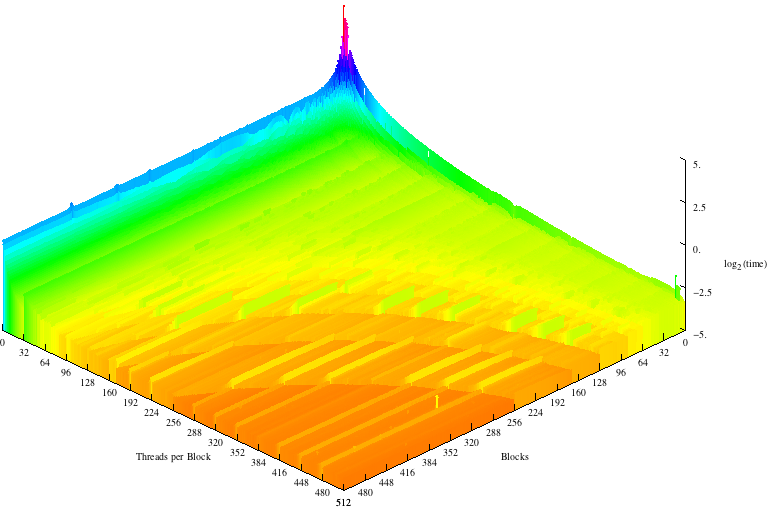
\includegraphics{MediumPlot.png}
\end{figure}

There are a number of interesting things to note about this
graph:
\begin{itemize}
\item {} 
Trials with one block and many threads are faster than
trials with many blocks of one thread each.

\item {} 
There are horizontal lines indicating a spike in execution
time after every 32 threads per block

\item {} 
512 threads per 512 blocks was the fastest execution time

\item {} 
There are convex lines running through the middle of the
graph

\end{itemize}

Each of these observations relates directly to CUDA's
architecture or the specifics of the code.

Many threads in 1 block is always faster than many blocks of
one thread because of the way threads are put into warps.
The Jetson can execute 4 warps simultaneously. This means that
when the number of threads/block is one only 4 threads can run concurently
but when the number of blocks is one and there are many threads per block,
the threads can be evenly divided
into warps so that up to 128 are being run simultaneously.

Warp size also explains the horizontal lines every
32 threads per block. When block are are evenly divisible
into warps of 32, each block uses the full resources of the
CUDA cores on which it is run, but when there are (32 * x) +
1 threads, a whole new warp must be scheduled for a single
thread which wastes 31 cycles cycles per block.

512x512 is the fastest execution time even though the GPU
can't run that many threads at a time. This is because
it is inexpensive to create threads on a CUDA card and having
one pixel per thread allows the GPU to
most efficently schedule warps as the CUDA cores become free.
Additionally, since accessing the color data takes time, the
GPU can help us out by calculating other warps while waiting
for the read to finish.

The convex lines appear for a few different reasons. The
first has to do with our code. When the picture is evenly
divisible by the total number of threads and blocks, each
thread performs the same amount of work so the warps aren't
bogged down by the threads that calculate the extra pixels.
Second, when block and grid dimensions are about roughly
equal, the block and warp schedulers share the work of
dividing the threads.


\section{Adding More Streaming Multiprocessors}
\label{2-Findings/Findings:adding-more-streaming-multiprocessors}
We executed our code again on a GeForce GTX 480 card that
has 15 SMs with 32 CUDA cores each.
\begin{figure}[htbp]
\centering

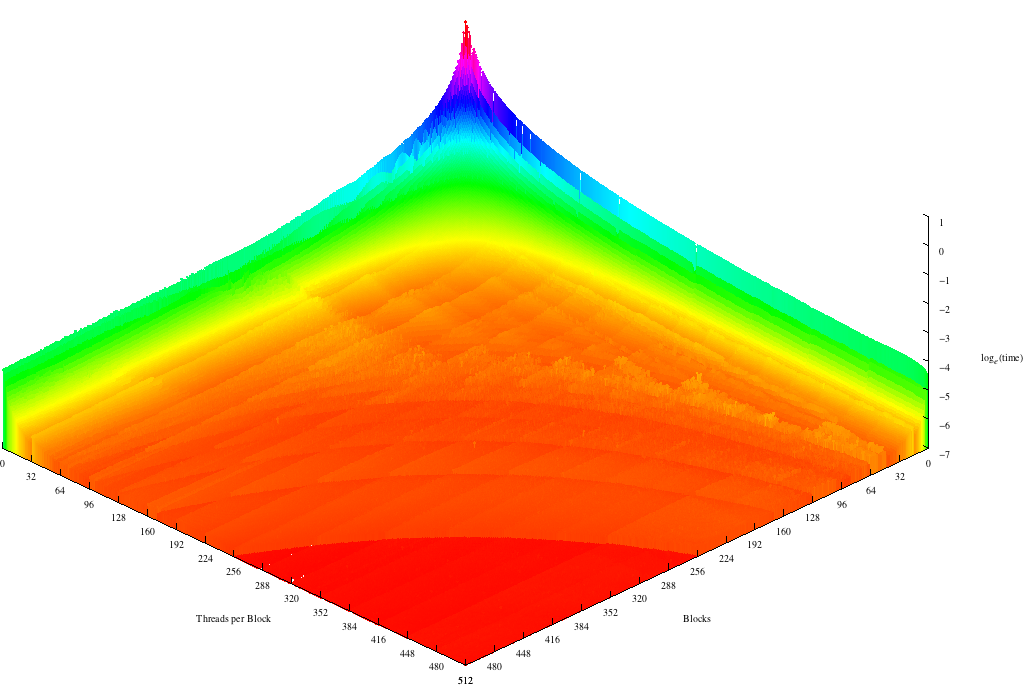
\includegraphics{Dev0Medium.png}
\end{figure}

This graph also features horizontal lines at multiples of
32 coresponding to the warp size, concave lines, and a top
execution speed at 512x512. However there are 2 important
differences.

First, one block of many threads and many blocks with one
thread each take about the same amount of time to execute.
Because this card uses the Fermi architecture, each SM can run
two warps concurently, this means that 64 threads can be running
at any given time. While still not as fast as using one block,
many blocks is significantly faster with multiple SMs.

The second difference is a series of valleys running
perpendicular to the warp lines about every 15 blocks.
These valleys come from the way blocks are distributed
between the SMs. When the block size is a multiple of the
number of SMs, each processor will do the about same
amount of work. However, as the number of blocks increases
this difference becomes less and less important because
the blocks don't all take the same amount of time to execute
and so it's possible for three blocks to execute on one SM
in the time it takes for another to execute 2.


\section{CUDA best practices}
\label{2-Findings/Findings:cuda-best-practices}
From these results we can draw up a list of best practices:
\begin{enumerate}
\item {} 
Try to make the number of threads per block a multiple of 32.

\item {} 
Keep the number of threads per block and the number of blocks as close to equal as you can without violating the first tip.

\item {} 
Keep the amount of work each thread does constant, it's inefficent to have one thread perform calculations for two pixels while the rest only calculate one.

\item {} 
When in doubt use more threads not less, creating threads is inexpensive.

\item {} 
In general avoid having threads that do extra work or have conditionals.

\item {} 
Try to have a block size that is a multiple of the numberof SMs on your device, this is less important than the other tips.

\end{enumerate}



\renewcommand{\indexname}{Index}
\printindex
\end{document}
